\section*{Analyse}
\label{Analyse}
%
Analysen foretages på datasættet, som er præsenteret i \autoref{fig:Data} og indeholder sammenligningsdata for vurderingen af ansigtsudtrykkene. 
%
\begin{figure}[H]
\centering
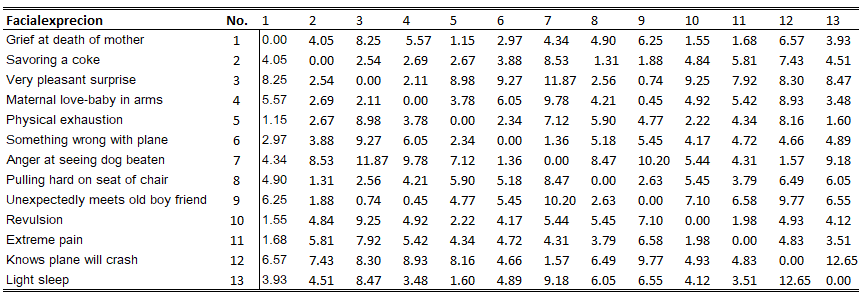
\includegraphics[width = \textwidth]{Figure/Data.PNG} 
\caption{Sammenligning mellem vurderingen af de 13 ansigtsudtryk, hvor 0 indikerer, at ansigtsudtrykkene er vurderet helt ens.}
\label{fig:Data}
\end{figure}
\noindent
%
\autoref{fig:Data} giver ikke et specielt godt overblik over sammenhæng og forskellen mellem vurderingerne af ansigtsudtrykkene. For at få et overblik udføres der en \textit{Non-metric MDS}, som beskrevet er beskrevet i \fullref{Metode}. 
\vfill
\subsection*{Valg af dimensioner}
%
Første step er at bestemme det optimale antal dimensioner. Måden hvorpå det gøres, er ved lave et \textit{Scree}-plot, hvor sammenhængen mellem \textit{stress} og antal dimensioner kan aflæses ud fra. Plottet er præsenteret på \autoref{fig:ScreePlot}. 
%
\begin{figure}[H]
\centering
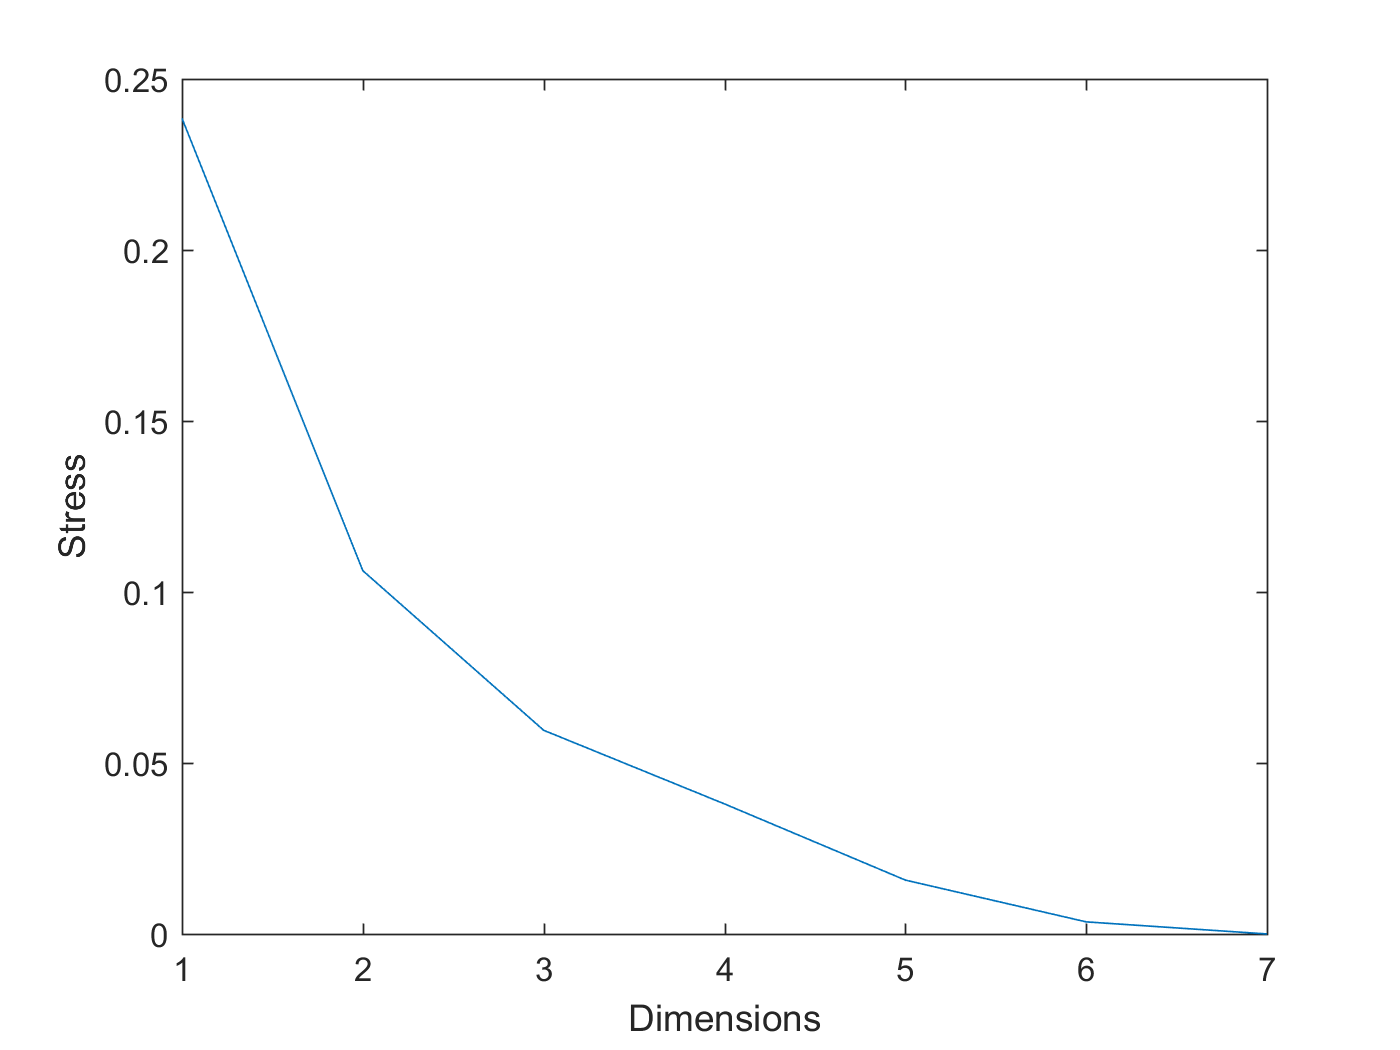
\includegraphics[width = 0.8\textwidth]{Figure/screeplot.png} 
\caption{\textit{Scree}-plot: Forholdet mellem \textit{stress} og antallet af dimensioner. Det forekommer to markante albue-punkter ved henholdvis to og tre dimensioner.}
\label{fig:ScreePlot}
\end{figure}
\noindent
%
\textit{Scree}-plottet har forskellige albue-punkter (\textit{elbow-points}), som er de steder, hvor kurven knækker. Det er ud fra disse punkter at antallet af dimensioner bestemmes afhængigt af \textit{stress}-værdien. Mindskes \textit{stress}-værdien er det nødvendigt med flere dimensioner.\blankline  
%
Antallet af dimensioner vælges til at være to, der har en \textit{stress}-værdi på 0,1062. Dette antal dimensioner er det første albue-punkt på \textit{Scree}-plottet, jævnfør \autoref{fig:ScreePlot}, derudover er \textit{stress}-værdien acceptabel, da den svarer til \textit{fair}, jævnfør \autoref{fig:TolkningStress}. Ydermere mindskes \textit{stress} betydeligt ved at gå fra én dimension til to, hvor \textit{stress} ikke mindskes lige så meget ved at øge antallet af dimensioner. Det er også vigtigt for valget af dimensioner, at skalaen bliver lettere at fortolke og arbejde med, hvilket gør sig gældende for to dimensioner. Det betyder, at \textit{stress} ved tre dimensioner er mindre (0,0596), hvorfor der opnåes en bedre repræsentation af datapunkterne. Derudover er det lettere at fortolke to dimensioner, da det er svært at repræsentere tre dimensioner på et to dimensionelt papir. Forsøges det at repræsentere flere end tre dimensioner på et to dimensionelt plan, vil resultatet af MDS være tæt på ubrugeligt, særligt når hvis det  forsøges at tydeliggøre komplekse sammenhænge i datasættet, \parencite{Borgatti1997}. 

For at undersøge mere detaljeret, hvor godt de to dimensioner passer på datasættet udarbejdes der et \textit{Shepard}-plot, jævnfør \autoref{fig:ShepardPlot}.
%
\begin{figure}[H]
\centering
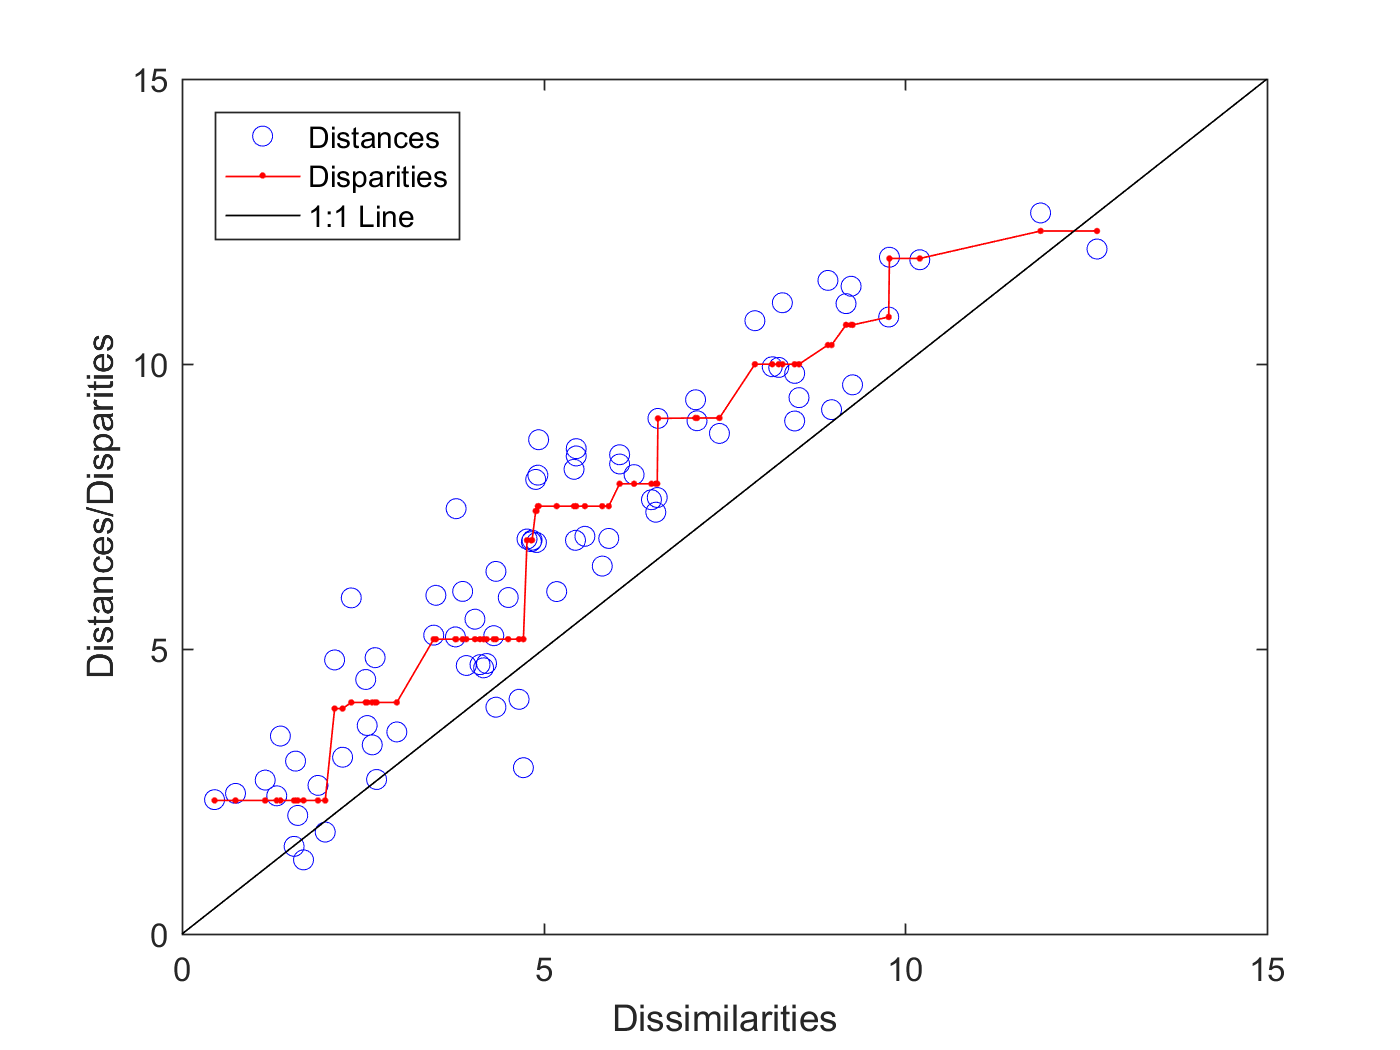
\includegraphics[width = 0.8\textwidth]{Figure/Sheppard_plot.png} 
\caption{\textit{Shepard}-plot: datapunkterne, angivet med cirkler, er fittet ud fra den røde kurve \textit{Disparities}, som sammenlignes med den diagonale sorte kurve.}
\label{fig:ShepardPlot}
\end{figure}
\noindent
%
På \autoref{fig:ShepardPlot} fremgår det, at det indsamlede data afviger fra det perfekte fit, som er den sorte linje \textit{1:1 Line}. Det vurderes, at afvigelsen, der er fra det perfekte fit, er lille nok til at fortsætte analysen med de valgte to dimensioner. 
%
\vfill

\subsection*{MDS-plot}
2-dimensionel \textit{non-metric MDS} for vurderingen af ansigtsudtrykkene præsenteres på \autoref{fig:MDS}.  
%
\begin{figure}[H]
\centering
\includegraphics[width =\textwidth]{Figure/MDS_plot} 
\caption{MDS af det perceptuelle rum i to dimensioner. Datapunkter, der ligger tæt på hinanden har en højere korrelation end datapunkter, der ligger langt fra hinanden. Dog er der større usikkerhed omkring punkter tæt på hinanden ift. punkter langt fra hinanden. Der er højere præcision jo længere væk punkterne er - data er bedre repræsenteret.}
\label{fig:MDS}
\end{figure}
\noindent
%
Baseret på \autoref{fig:MDS} samt placeringen af ansigtsudtrykkene heri, kan det undersøges hvilke labels de to dimensioner kan have for at det giver mening i forhold til hvordan ansigtsudtrykkene er placeret.\blankline 
%
Dimension 1, som er den vandrette akse (x-aksen) på plottet, kan være \textit{Negativitet}, på engelsk \textbf{Negativity}. Hvis værdien stiger vil personen være mere negativ. Hvis værdien er under nul, vil personen være mere positiv, som vurderes til at være det modsatte af negativ.\blankline
%
Dimension 2, som er den lodrette akse (y-aksen) på plottet, kan være \textit{Fraværende}, på engelsk \textbf{Absent-minded}. Hvis værdien stiger vil personen være mere fraværende. Hvis værdien er under nul, vil personen være mere tilstedeværende, som vurderes til at være det modsatte af fraværende. \blankline
%
Det kan ikke undgås, at der opstår afvigelser fra de tildelte labels, da der ved to dimensioner er en \textit{stress}-værdi på 0,1062, som gengiver at det ikke er et perfekt fit ved blot to dimensioner. Nogle punkter vil derfor være placeret tættere eller længere fra hinanden end den forskel, der reelt er.\blankline
%
På \autoref{fig:MDSA} er der tilføjet pile i forhold til fortolkningen, hvor hver pil repræsenterer én attribut. Længden og retningen af pilen indikerer henholdsvis, hvor godt den passer og hvornår den øges. Det er forfatternes egen fortolkning. 
%
\begin{figure}[H]
\centering
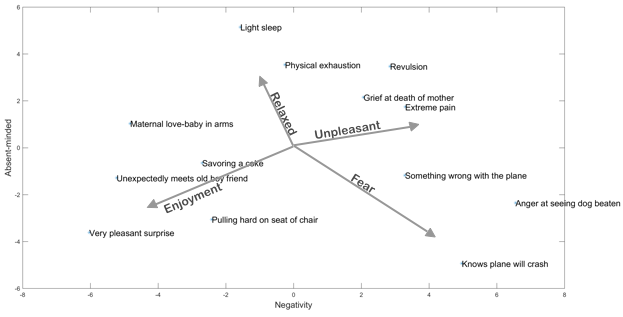
\includegraphics[width =\textwidth]{Figure/MSD_PlotArrows.png} 
\caption{MDS: to dimensioner, med indsatte retningsvektorer og labels.}
\label{fig:MDSA}
\end{figure}
\noindent
%